\documentclass{article}

% packages
  % basic stuff for rendering math
  \usepackage[letterpaper, top=1in, bottom=1in, left=1in, right=1in]{geometry}
  \usepackage[utf8]{inputenc}
  \usepackage[english]{babel}
  \usepackage{amsmath} 
  \usepackage{amssymb}
  % \usepackage{amsthm}

  % extra math symbols and utilities
  \usepackage{mathtools}        % for extra stuff like \coloneqq
  \usepackage{mathrsfs}         % for extra stuff like \mathsrc{}
  \usepackage{centernot}        % for the centernot arrow 
  \usepackage{bm}               % for better boldsymbol/mathbf 
  \usepackage{enumitem}         % better control over enumerate, itemize
  \usepackage{hyperref}         % for hypertext linking
  \usepackage{fancyvrb}          % for better verbatim environments
  \usepackage{newverbs}         % for texttt{}
  \usepackage{xcolor}           % for colored text 
  \usepackage{listings}         % to include code
  \usepackage{lstautogobble}    % helper package for code
  \usepackage{parcolumns}       % for side by side columns for two column code
  

  % page layout
  \usepackage{fancyhdr}         % for headers and footers 
  \usepackage{lastpage}         % to include last page number in footer 
  \usepackage{parskip}          % for no indentation and space between paragraphs    
  \usepackage[T1]{fontenc}      % to include \textbackslash
  \usepackage{footnote}
  \usepackage{etoolbox}

  % for custom environments
  \usepackage{tcolorbox}        % for better colored boxes in custom environments
  \tcbuselibrary{breakable}     % to allow tcolorboxes to break across pages

  % figures
  \usepackage{pgfplots}
  \pgfplotsset{compat=1.18}
  \usepackage{float}            % for [H] figure placement
  \usepackage{tikz}
  \usepackage{tikz-cd}
%  \usepackage{circuit-tikz}
  \usetikzlibrary{arrows}
  \usetikzlibrary{positioning}
  \usetikzlibrary{calc}
  \usepackage{graphicx}
  \usepackage{caption} 
  \usepackage{subcaption}

  % for tabular stuff 
  \usepackage{dcolumn}

  \usepackage[nottoc]{tocbibind}
  \pdfsuppresswarningpagegroup=1
  \hfuzz=5.002pt                % ignore overfull hbox badness warnings below this limit

% New and replaced operators
  \DeclareMathOperator{\Tr}{Tr}
  \DeclareMathOperator{\Sym}{Sym}
  \DeclareMathOperator{\Span}{span}
  \DeclareMathOperator{\std}{std}
  \DeclareMathOperator{\Cov}{Cov}
  \DeclareMathOperator{\Var}{Var}
  \DeclareMathOperator{\Corr}{Corr}
  \DeclareMathOperator{\pos}{pos}
  \DeclareMathOperator*{\argmin}{\arg\!\min}
  \DeclareMathOperator*{\argmax}{\arg\!\max}
  \newcommand{\ket}[1]{\ensuremath{\left|#1\right\rangle}}
  \newcommand{\bra}[1]{\ensuremath{\left\langle#1\right|}}
  \newcommand{\braket}[2]{\langle #1 | #2 \rangle}
  \newcommand{\qed}{\hfill$\blacksquare$}     % I like QED squares to be black

% Custom Environments
  \newtcolorbox[auto counter, number within=section]{question}[1][]
  {
    colframe = orange!25,
    colback  = orange!10,
    coltitle = orange!20!black,  
    breakable, 
    title = \textbf{Question \thetcbcounter ~(#1)}
  }

  \newtcolorbox[auto counter, number within=section]{exercise}[1][]
  {
    colframe = teal!25,
    colback  = teal!10,
    coltitle = teal!20!black,  
    breakable, 
    title = \textbf{Exercise \thetcbcounter ~(#1)}
  }
  \newtcolorbox[auto counter, number within=section]{solution}[1][]
  {
    colframe = violet!25,
    colback  = violet!10,
    coltitle = violet!20!black,  
    breakable, 
    title = \textbf{Solution \thetcbcounter}
  }
  \newtcolorbox[auto counter, number within=section]{lemma}[1][]
  {
    colframe = red!25,
    colback  = red!10,
    coltitle = red!20!black,  
    breakable, 
    title = \textbf{Lemma \thetcbcounter ~(#1)}
  }
  \newtcolorbox[auto counter, number within=section]{theorem}[1][]
  {
    colframe = red!25,
    colback  = red!10,
    coltitle = red!20!black,  
    breakable, 
    title = \textbf{Theorem \thetcbcounter ~(#1)}
  } 
  \newtcolorbox[auto counter, number within=section]{proposition}[1][]
  {
    colframe = red!25,
    colback  = red!10,
    coltitle = red!20!black,  
    breakable, 
    title = \textbf{Proposition \thetcbcounter ~(#1)}
  } 
  \newtcolorbox[auto counter, number within=section]{proof}[1][]
  {
    colframe = orange!25,
    colback  = orange!10,
    coltitle = orange!20!black,  
    breakable, 
    title = \textbf{Proof. }
  } 
  \newtcolorbox[auto counter, number within=section]{definition}[1][]
  {
    colframe = yellow!25,
    colback  = yellow!10,
    coltitle = yellow!20!black,  
    breakable, 
    title = \textbf{Definition \thetcbcounter ~(#1)}
  } 
  \newtcolorbox[auto counter, number within=section]{example}[1][]
  {
    colframe = blue!25,
    colback  = blue!10,
    coltitle = blue!20!black,  
    breakable, 
    title = \textbf{Example \thetcbcounter ~(#1)}
  } 
  \newtcolorbox[auto counter, number within=section]{code}[1][]
  {
    colframe = green!25,
    colback  = green!10,
    coltitle = green!20!black,  
    breakable, 
    title = \textbf{Code \thetcbcounter ~(#1)}
  } 

  \BeforeBeginEnvironment{example}{\savenotes}
  \AfterEndEnvironment{example}{\spewnotes}
  \BeforeBeginEnvironment{lemma}{\savenotes}
  \AfterEndEnvironment{lemma}{\spewnotes}
  \BeforeBeginEnvironment{theorem}{\savenotes}
  \AfterEndEnvironment{theorem}{\spewnotes}
  \BeforeBeginEnvironment{corollary}{\savenotes}
  \AfterEndEnvironment{corollary}{\spewnotes}
  \BeforeBeginEnvironment{definition}{\savenotes}
  \AfterEndEnvironment{definition}{\spewnotes}
  \BeforeBeginEnvironment{exercise}{\savenotes}
  \AfterEndEnvironment{exercise}{\spewnotes}
  \BeforeBeginEnvironment{proof}{\savenotes}
  \AfterEndEnvironment{proof}{\spewnotes}
  \BeforeBeginEnvironment{solution}{\savenotes}
  \AfterEndEnvironment{solution}{\spewnotes}
  \BeforeBeginEnvironment{question}{\savenotes}
  \AfterEndEnvironment{question}{\spewnotes}
  \BeforeBeginEnvironment{code}{\savenotes}
  \AfterEndEnvironment{code}{\spewnotes}

  \definecolor{dkgreen}{rgb}{0,0.6,0}
  \definecolor{gray}{rgb}{0.5,0.5,0.5}
  \definecolor{mauve}{rgb}{0.58,0,0.82}
  \definecolor{lightgray}{gray}{0.93}

  % default options for listings (for code)
  \lstset{
    autogobble,
    frame=ltbr,
    language=C,                           % the language of the code
    aboveskip=3mm,
    belowskip=3mm,
    showstringspaces=false,
    columns=fullflexible,
    keepspaces=true,
    basicstyle={\small\ttfamily},
    numbers=left,
    firstnumber=1,                        % start line number at 1
    numberstyle=\tiny\color{gray},
    keywordstyle=\color{blue},
    commentstyle=\color{dkgreen},
    stringstyle=\color{mauve},
    backgroundcolor=\color{lightgray}, 
    breaklines=true,                      % break lines
    breakatwhitespace=true,
    tabsize=3, 
    xleftmargin=2em, 
    framexleftmargin=1.5em, 
    stepnumber=1
  }

% Page style
  \pagestyle{fancy}
  \fancyhead[L]{Measure Theory}
  \fancyhead[C]{Muchang Bahng}
  \fancyhead[R]{Fall 2022} 
  \fancyfoot[C]{\thepage / \pageref{LastPage}}
  \renewcommand{\footrulewidth}{0.4pt}          % the footer line should be 0.4pt wide
  \renewcommand{\thispagestyle}[1]{}  % needed to include headers in title page

\begin{document}

\title{Measure Theory}
\author{Muchang Bahng}
\date{Spring 2024}

\maketitle
\tableofcontents
\pagebreak

In math, we are first taught to solve simple equations like $x^2 - 2x + 4 = 0$ for a certain \textit{number} $x$, but in real world applications, we must now solve for some \textit{function} $f$ satisfying an equation 
\[\mathcal{L}(f) = 0\]
where $\mathcal{L}$ is some operator on functions. This is usually difficult, and many times a solution does not exist. However, we can find approximate solutions, say 
\begin{align*}
    \mathcal{L}(f) & = 1/2 \\
    \mathcal{L}(f) & = 1/4 \\ 
    \mathcal{L}(f) & = 1/8 \\
    \ldots & = \ldots 
\end{align*}
and approximate the solution as 
\[f = \lim_{n \rightarrow \infty} f_n \]
Given that this limit exists, we can usually define $f$ pointwise using a point-wise limit 
\[f(x) = \lim_{n \rightarrow \infty} f_n (x) \text{ for all } x\]
but the function in total is very ugly and not Riemann integrable. The classic non-Riemann integrable function is the 
\[f(x) = \chi_{\mathbb{R} \setminus \mathbb{Q}} (x) \coloneqq \begin{cases} 
1 & \text{ if } x \in \mathbb{R} \setminus \mathbb{Q} \\
0 & \text{ if} x \in \mathbb{Q} 
\end{cases}\]
Since $\mathbb{Q}$ is countable, we can enumerate $\mathbb{Q} = \{q_n\}_{n=1}^\infty$ and define the sequence of functions 
\[f_n = 1 - \chi_{\{q_j\}_{j=1}^n}(x)\]
that start off with the constant function $1$ and then "removes" points in $\mathbb{Q}$, setting their image to $0$. It is clear that since we are removing points, every function in the sequence has an integral (from $0$ to $1$) of $1$, and therefore the integral of $f$ should also be $1$. 
\[\int_0^1 f_n \, dx = 1 \implies \int_0^1 f \,dx = \int_0^1 \lim_{n \rightarrow \infty} f_n \,dx = \lim_{n \rightarrow \infty} \int_0^1 f_n \,dx\]
What is crucial for mathematicians to work with is the capability to take the limit from inside the integral to outside the integral. The problem is that $f$ is not a Riemann integral function. 

\begin{definition}[Riemann Integrable Function]
Given a function $f: [0, 1] \longrightarrow \mathbb{R}$, let us consider some partition of $[0, 1]$ into intervals $P = \{I_0, I_1, \ldots, I_N\}$, then, for each $I \in P$, we can take the supremum $M_I = \sup_{x \in I} f(x)$ and infimum $m_I = \inf_{x \in I} f(x)$ and bound $f$ by the upper and lower Riemann sums. 
\[\sum_{I \in P} m_I |I| \leq \int_0^1 f \,dx \leq \sum_{I \in P} M_I |I| \]
where $|I|$ is the length of interval $I$. If we take \textit{all} possible partitions, the bound should still hold. 
\[m = \sup_P \Big\{ \sum_{I \in P} m_I |I| \Big\} \leq \int_0^1 f \,dx \leq \inf_P \Big\{ \sum_{I \in P} M_I |I| \Big\} = M\]
and if the lower bound is equal to the upper bound $m = M$, then the integral is this number and $f$ is considered Riemann integrable. 
\end{definition}

Now since $\mathbb{Q}$ is dense in $\mathbb{R}$, for every interval $I$ in every partition $P$ will have $m_I = 0$ and $M_I = 1$ for the Riemann function, meaning that the lower bound will always be $0$ and the upper bound will always be $1$. So, $\int_0^1 \chi_{\mathbb{R} \setminus \mathbb{Q}} (x)$ can take on any value in $[0, 1]$, which isn't helpful. The fact that we can't integrate this really simple function is a problem. For nice functions, we can partition it so that the base of each Riemann rectangle is a nice interval, while the base of the Riemann function is an "interval with holes." The problem really boils down to measuring what the "length" of this set is. So the problem with the Riemann integral isn't the integral itself, but the fact that we can't give a meaningful size to the set $\mathbb{R} \setminus \mathbb{Q}$. Now mathematicians in the 19th century thought that as long as we solve this problem, we should be good to go, but Banach and Tarski proved that there exists sets that cannot be measured with their famous paradox, which says that you can take any set $P$, disassemble it into a finite set of pieces, and rearrange it (under isometry and translations) so that it has a different size than the original $P$. So, we have to exclude some sets that are not measurable. The collection of sets that we \textit{can} measure is called the $\sigma$-algebra. 

\section{Measures and Sigma Algebras}

Now, given any set $X$, we can construct its power set $2^X$. But we can't naively just give a measure to every $A \in 2^X$, since for certain spaces, this causes nasty contradictions shown through the Banach-Tarski Paradox. 

\begin{theorem}[Banach-Tarski Paradox (Strong Form)]
Given any two bounded subsets $A$ and $B$ of $\mathbb{R}^n$ where $n \geq 3$, both of which have a nonempty interior, there are partitions of $A$ and $B$ into a finite number of disjoint subsets, $A = A_1 \cup \ldots \cup A_k$, $B = B_1 \cup \ldots \cup B_k$, such that $A_i$ and $B_i$ are congruent for every $i \in [k]$. 
\end{theorem}

A nice set of subsets of $X$ to work with is the $\sigma$-algebra of $X$. 

\begin{definition}[$\sigma$-Algebra]
A \textbf{$\boldsymbol{\sigma}$-algebra} on a set $X$ is a collection  of subsets of $X$, denoted $\mathcal{A} \subset 2^X$ that contains $\emptyset$, $X$ itself, is stable under a countable union, and is stable under complementation. This pair $(X, \mathcal{A})$ is called a \textbf{measurable space}. 
\end{definition}

\begin{lemma}[Additional Property of $\sigma$-Algebras]
A commonly known property of any $\sigma$-algebra $\mathcal{A}$ is that it is stable under countable intersections, too. 
\[A_1, A_2, \ldots, \in \mathcal{A} \implies \bigcap_{k=1}^\infty A_k \in \mathcal{A}\]
\end{lemma}
\begin{proof}
We can utilize the fact that 
\[\bigcap_{k=1}^\infty A_k = X \setminus \bigcup_{k=1}^\infty A_k^c\]
\end{proof}

A $\sigma$-algebra is similar to the topology $\tau$ of topological space. Both $\mathcal{A}$ and $\tau$ require $\emptyset$ and $X$ to be in it. The three differences are that (i) $\tau$ does not allow compelmentation, (ii) $\tau$ allows any (even uncountable) union of sets (condition is strengthened), and (iii) $\tau$ allows only finite intersection of sets (condition is weakened). Now in order to construct $\sigma$-algebras, the following theorems are useful since they allow us to construct $\sigma$-algebras from other $\sigma$-algebras. It turns out that the intersection of $\sigma$-algebras is a $\sigma$-algebra, but not for unions. 

\begin{theorem}[Intersection of Sigma Algebras is a Sigma Algebra]
  Let $\{\mathcal{A}_k\}$ be a family of $\sigma$-algebras of $X$. Then, $\cap \mathcal{A}_k$ is also a $\sigma$-algebra of $X$. 
\end{theorem}
\begin{proof}
  Clearly, $\emptyset, X$ is in $\cap \mathcal{A}_k$. To prove complementation, 
  \begin{equation}
    A \in \bigcap \mathcal{A}_k \implies A \in \mathcal{A}_k \; \forall k \implies A^c \in A_k \; \forall k \implies A^c \in \bigcap \mathcal{A}_k
  \end{equation}
  To prove countable union, let $\{A_j\}_{j \in J}$ be some countable family of subsets in $\cap \mathcal{A}_k$. Then, 
  \begin{equation}
    A_j \in \bigcap \mathcal{A}_k \; \forall j \in J \implies A_j \in \mathcal{A}_k \; \forall k \forall j \implies \bigcup A_j \in \mathcal{A}_k \; \forall k \implies \bigcup A_j \in \bigcap \mathcal{A}_k
  \end{equation}
\end{proof}

This allows us to easily prove the following proposition, which just establishes the existence of $\sigma$-algebras. 

\begin{proposition}[Unique Smallest Sigma Algebra]
  Let $F \subset 2^X$. Then there exists a unique smallest $\sigma$-algebra $\sigma(F)$ containing $F$. 
\end{proposition}
\begin{proof}
  Let us denote $\mathcal{M}$ as the set of all possible $\sigma$-algebras $\mathcal{B}$ of $X$. $\mathcal{M}$ is nonempty since it contains $2^X$. Then, the intersection 
  \[\bigcap_{\mathcal{B} \in \mathcal{M}} \mathcal{B}\]
  is the unique smallest $\sigma$-algebra. 
\end{proof}

Now, we can introduce the first nontrivial $\sigma$-algebra, called the Borel $\sigma$-algebra. 

\begin{definition}[Borel $\sigma$-algebra]
  The \textbf{Borel $\boldsymbol{\sigma}$-algebra} of a topological space $(X, \tau)$ is the $\sigma$-algebra generated by the topology $\tau$, denoted $\mathcal{B}(X)$. 
\end{definition}

Now, how do we measure a size on $\mathcal{B}(X)$? We use measures. 

\begin{definition}[Measure]
  Given a measurable space $(X, \mathcal{A})$, a \textbf{measure} is a function $\mu : \mathcal{A} \longrightarrow [0, +\infty]$ satisfying 
  \begin{enumerate}
    \item Null empty set $\mu(\emptyset) = 0$ 
    \item Countable additivity: For all countable collections $\{A_k\}_{k=1}^\infty$ of pairwise disjoint subsets $A_k \in \mathcal{A}$, 
    \[\mu \bigg( \bigsqcup_{k=1}^\infty A_k \bigg) = \sum_{k=1}^\infty \mu(A_k)\]
    Remember that we are allowed to take countable unions inside our $\sigma$-algebra, so this makes sense. 
  \end{enumerate}
  This immediately implies that given $A, B \in \mathcal{A}$, then $A \subset B \implies \mu(A) \leq \mu(B)$. The triplet $(X, \mathcal{A}, \mu)$ is called a \textbf{measure space}. 
\end{definition}

The first condition is important because it allows us to take finite disjoint unions. That is, since $\mu(A_1 \cup A_2) = \mu(A_1 \cup A_2 \cup \emptyset \cup \ldots)$, we have 
\[\sum_{k=1}^\infty = \mu(A_1) + \mu(A_2)\]
Disjointness is clearly important since if it wasn't, then $\mu(A) = \mu(A \cup A) = 2 \mu(A)$, which is absurd. Now our natural measure on the real number line with its Borel $\sigma$-algebra $(\mathbb{R}, \mathcal{B})$, we want a measure satisfying $\mu((a, b)) = b - a$ and $\mu([0, \infty)) = \infty$. Such a measure does exist, and it is called the Lebesgue measure, but proving its existence is highly nontrivial. Let us first look into some properties of measures, which all seem natural. 

\begin{proposition}
  If $A_1 \subset A_2 \subset A_3 \subset \ldots$, then 
  \[\mu\bigg( \bigcup_{k=1}^\infty A_k \bigg) = \lim_{k \rightarrow \infty} \mu(A_k)\]
\end{proposition}
\begin{proof}
  This is the first time we introduce limits. With the fact that $\mu(A_k)$ must be nondecreasing, we can use real analysis and see that it is bounded by $\infty$, meaning that it must have a limit. But why does this limit equal to the left hand side? We can see that 
  \begin{align}
    \mu\bigg( \bigcup_{k=1}^\infty A_k \bigg) & = \mu(A_1) + \sum_{k=2}^\infty \mu(B_k) \\
    & = \mu(A_1) + \lim_{k \rightarrow \infty} \sum_{k=2}^\infty \mu(B_k) \\
    & = \lim_{k \rightarrow \infty} \mu(A_1 \cup B_2 \cup \ldots B_k)  = \lim_{k \rightarrow \infty} \mu(A_k) 
  \end{align}
  where $B_k = A_k \setminus A_{k-1}$. 
\end{proof}

Now a similar theorem, but with a little twist to it. 

\begin{proposition}
  If $A_1 \supset A_2 \supset A_3 \supset \ldots$, then 
  \[\mu\bigg( \bigcap_{k=1}^\infty A_k \bigg) = \lim_{k \rightarrow \infty} \mu(A_k)\]
  if $\mu(A_1) < \infty$. 
\end{proposition}
\begin{proof}
  The $\mu(A_1) < \infty$ is a necessary condition, since if we take $A_k = [k, \infty)$ on the real number line, then we have $\cap_{k=1}^\infty A_k = \emptyset$, but the limit of the measure is $\infty$. Well we can define $B_k = A_k \setminus A_{k+1}$ and write $\cap_{k=1}^\infty A_k = A_1 \setminus \cup_{k=1}^\infty B_k$, which means that 
  \begin{align*}
    \mu\bigg( \bigcap_{k=1}^\infty A_k \bigg) & = \mu\bigg( A_1 \setminus \bigcup_{k=1}^\infty B_k \bigg) \\
    & = \mu(A_1) - \mu\bigg( \bigcup_{k=1}^\infty B_k\bigg) \\
    & = \mu(A_1) - \sum_{k=1}^\infty \mu(B_k) \\
    & = \mu(A_1) - \lim_{K \rightarrow \infty} \sum_{k=1}^K \mu(B_k) \\
    & = \lim_{K \rightarrow \infty} \bigg( \mu(A_1) - \sum_{k=1}^K \mu(B_k) \bigg) \\
    & = \lim_{K \rightarrow \infty} \mu \bigg( A_1 \setminus \bigcup_{k=1}^K B_k \bigg) = \lim_{K \rightarrow \infty} \mu(A_K)
  \end{align*}
  Now the first line uses the fact that if $A \subset B$, then $\mu(B \setminus A) + \mu(A) = \mu(B)$, and with the further assumption that $\mu(A) < \infty$, we can subtract on both sides like we do with regular arithmetic. 
\end{proof}

\subsection{Outer Measures, Construction of Lebesgue Measure}

Now let's try to construct a measure $\lambda$ on the Borel $\sigma$-algebra $\mathcal{B}(\mathbb{R})$ that assigns length, i.e. $\lambda([a, b]) = b - a$. We will do so by constructing outer measures $\lambda^*: 2^\mathbb{R} \longrightarrow \mathbb{R}$ that acts on the power set of $\mathbb{R}$ s.t. $\lambda^*([a, b]) = b - a$. But this turns out to have its own problems and contradictions, so once we construct such a $\lambda^*$, we will "throw away" all the sets that don't behave nicely under $\lambda^*$ and just use its restriction on the Borel algebra. It turns out that the sets that do behave well under $\lambda^*$ is bigger than the Borel algebra, call it $\mathcal{M}_{\lambda^*}$. So, we have $\mathcal{B}(\mathbb{R}) \subset \mathcal{M}_{\lambda^*} \subset 2^\mathbb{R}$. We will do this in full generality in the following way. We take any space $X$ and construct an outer measure $\mu^*$ on its power set $2^X$. Then, we construct the $\sigma$-algebra of well-behaved sets $\mathcal{M}_{\mu^*} \subset 2^X$, and define our measure $\mu$ on $\mathcal{M}_{\mu^*}$. When defining our outer measure, the condition that the outer measure of a disjoint union of subsets is equal to the sum of the outer measure of the subsets is a bit too restricting, so we use a softer condition. 

\begin{definition}[Outer Measure]
  A function $\mu^* : 2^X \longrightarrow [0, \infty]$ is an \textbf{outer measure} if $\mu^*(\emptyset) = 0$, $A \subset B \implies \mu^* (A) \leq \mu^*(B)$, and 
  \[\mu^* \bigg( \bigcup_{k=1}^\infty A_k \bigg) \leq \sum_{k=1}^\infty \mu^* (A_k)\]
  This final condition removes the fact that they must be disjoint, and now we have an inequality. 
\end{definition}

Now to construct our Lebesgue outer measure, let us define the following on $\mathbb{R}$. It's a hard definition, but a natural one, since we're taking all these intervals and trying to make them as snug as possible to define the outer measure of an arbitrary set. 

\begin{definition}[Lebesgue Outer Measure of $\mathbb{R}$]
  Given $A \subset \mathbb{R}$, let 
  \[C_A = \big\{ \{(a_j, b_j)\}_{j=1}^\infty \mid A \subset \bigcup_{j=1}^\infty (a_j, b_j) \big\}\]
  This is more complicated than it looks. Given a set $A$, we are looking at a family of all collections of intervals that cover $A$. Clearly, all coverings in $C_A$ must have a length greater than $A$, and their length can be easily measured by summing up the intervals $\sum_{j=1}^\infty (b_j - a_j)$. So, we can define the outer measure of $A$ to be the infimum of these sums. 
  \[\lambda^*(A) = \inf_{C_A} \sum_{j=1}^\infty (b_j - a_j)\]
  We can also generalize this further by introducing a increasing, continuous function $F: \mathbb{R} \rightarrow \mathbb{R}$ and defining the outer measure to be 
  \[\lambda^*(A) = \inf_{C_A} \sum_{j=1}^\infty \big( F(b_j) - F(a_j) \big) \]
\end{definition}

\begin{example}[Rationals have Outer Measure $0$]
  Let us prove that $\lambda^*(\mathbb{Q}) = 0$. It is countable so we can enumerate it $\mathbb{Q} = \{ q_j\}_{j=1}^\infty$. This is counterintuitive, because since $\mathbb{Q}$ is dense in $\mathbb{R}$, in order to make a covering of $\mathbb{Q}$ we sort of have to cover the entire real line. Visually, this is hard, but it is pretty simple to show that you don't have to. We pick $\epsilon > 0$ and define 
  \[I_j = \big( q_j - \frac{\epsilon}{2^j} , q_j + \frac{\epsilon}{2^j} \big)\]
  So, 
  \[\sum_{j=1}^\infty |I_j| = \sum_{j=1}^\infty \frac{\epsilon}{2^j} = 2 \epsilon\]
  This collection $\{I_j\}$ is one element of $C_\mathbb{Q}$ of coverings of the rationals, and taking $\epsilon$ as small as we want, the infimum is $0$. This can be done with all countable subsets of $\mathbb{R}$. 
\end{example}

\begin{definition}[Almost Everywhere]
  Given a measure space $(X, \mathcal{A}, \mu)$, a subset $A \in \mathcal{A}$ is said to be a $\mu$-null set if $\mu(A) = 0$. If some property holds for all points $x \in X$ except on a null set, then we say that the property holds \textbf{almost everywhere}.
\end{definition}

\begin{example}[Rational Function]
  The function $f(x) = \frac{1}{\sqrt{|x|}}$ is less than $\infty$ almost everywhere. 
\end{example}

\begin{proposition}[$\lambda^*$ is an Outer Measure]
  The first condition is trivial. As for 2, if I have $A \subset B \subset \mathbb{R}$ and have a covering of $B$, then I also have a covering of $A$, and so the infimum corresponding to the covering of $B$ must be greater than or equal to the infimum of that corresponding to the covering of $A$. For 3, we want to prove that the outer measure of the union of $A_k$'s is less than or equal to the sum of the outer measures of the $A_k$'s. We pick $\epsilon > 0$ and have some covering $\{(a^k_j, b^k_j)\}_{j=1}^\infty \in C_{A^k}$. So we have 
  \[\lambda^*(A_k) \leq \sum_{j=1}^\infty b^k_j - a^k_j\]
  We want the inequality to go the other way around, but we can't do that. But note that $\lambda^* (A_k)$ is the infimum of all coverings $\{(a^k_j, b^k_j)\}_{j=1}^\infty$ of $A_k$, and so we can choose a covering that is as close to $\lambda^* (A_k)$, and then add a term of $\epsilon$ to $\lambda^*(A_k)$ to make it greater than this covering. This is an important step of the proof that is used often! 
  \[\frac{\epsilon}{2^k} + \lambda^* (A_k) \geq \sum_{j=1}^\infty b_j^k - a_j^k \]
  Now, 
  \[A = \bigcup_{k=1}^\infty A_k \subset \bigcup_{k=1}^\infty \bigcup_{j=1}^\infty (a_j^k, b_j^k)\]
  and we can see that $\{(a_j^k , b_j^k)\}_{j, k=1}^\infty \in C_A$ is a countable covering of $A$ (since the countable union of a countable union is countable), implying that 
  \[\lambda^* (A) \leq \sum_{k=1}^\infty \sum_{j=1}^\infty (b_j^k - a_j^k) \leq \sum_{k=1}^\infty \bigg( \lambda^* (A_k) + \frac{\epsilon}{2^k} \bigg) = \epsilon + \sum_{k=1}^\infty \lambda^*(A_k)\]
  and so setting $\epsilon$ arbitrarily small we have $\lambda^* (A) \leq \sum_{k=1}^\infty \lambda^* (A_k)$. 
\end{proposition}

In $\mathbb{R}^n$, this construction is exactly the same, since we can take rectangular prisms, which we know the area/volume of, make a countable covering of some arbitrary set $A \subset \mathbb{R}^n$, and then find the infimum of the volume of this set. But we can't apply the outer measure on power sets since there exists some sets that do not behave like how we want it to behave under a measure. For example, there exists disjoint $A, B \subset (0, 1)$ s.t. $A \cup B = (0, 1)$, but $\lambda^*(A) + \lambda^*(B) > 1$. 

\begin{definition}[Carathéodory's criterion]
  Given outer measure $\mu^*$ on $X$, a set $B$ is $\mu^*$-measurable if 
  \[\forall A \subset X \; \mu^*(A) = \mu^*(A \cap B) + \mu^*(A \cap B^c)\]
  Obviously, the LHS $\leq$ RHS by the third condition of outer measures. 
\end{definition}

There is not much of an intuition for this definition, but in general it says that no matter how nasty a subset $A$ is, $B$ should be nice enough that we can cut $B$ into two pieces. Remember that this is a condition on $B$, not $A$. 

\begin{example}
  Take $X = \mathbb{R}$ and have $B = (-\infty, b]$. Then $B^c = (b, \infty)$, and $B$ divides $\mathbb{R}$ into a right side and a left side. If we take any subset $A \subset \mathbb{R}$, then $B$ is nice enough to divide $A$ into a left and a right side. 
\end{example}

\begin{theorem}
  If $\mu^*$ is an outer measure on $X$, $\mathcal{M}_{\mu^*} = \{$all $\mu^*$-measurable sets$\}$, then 
  \begin{enumerate}
    \item $\mathcal{M}_{\mu^*}$ is a $\sigma$-algebra. 
    \item $\mu = \mu^* \big|_{\mathcal{M}_{\mu^*}}$ is a measure. 
  \end{enumerate}
\end{theorem}

To recap, we first take a set $X$, construct an outer measure $\mu^*$ on it. This allows us to define the set of all $\mu^*$-measurable sets $B$ on $X$, which create a $\sigma$-algebra $\mathcal{M}$, and the restriction of $\mu^*$ onto $\mathcal{M}$ is a measure $\mu$. For $\mathbb{R}$, we can create our Lebesgue outer measure $\lambda^*$ on it, which generates the Lebesgue $\sigma$-algebra $\mathcal{M}_{\lambda^*}$. This turns out to be bigger than the Borel $\sigma$-algebra $\mathcal{B}(\mathbb{R})$, but there is little difference in which one we choose when we actually integrate. 

\begin{theorem}
  A set $E \subset \mathbb{R}$ is Lebesgue measurable implies that it is also Borel measurable. 
  \[\mathcal{B}(\mathbb{R}) \subset \mathcal{M}_{\lambda^*} \subset 2^\mathbb{R}\]
\end{theorem}

\begin{lemma}
  If $E \subset \mathbb{R}$ and $\lambda^*(E) = 0$, then $E \in \mathcal{M}_{\lambda^*}$, i.e. $E$ is Lebesgue outer-measurable. 
\end{lemma}
\begin{proof}
  We must prove that $E$ satisfies the Carathéodory's criterion. For all $E \subset \mathbb{R}$, we know that $\lambda^*(A) \leq \lambda^*(A \cap E) + \lambda^*(A \cap E^c)$ by definition of outer measure. Now, since $\lambda^* (E) =0$ and $A \cap E \subset E$, this means that $\lambda^* (A \cap E) = 0$ also. Furthermore, $A \cap E^c \subset A$, meaning that $\lambda^*(A) \geq \lambda^* (A \cap E^c)$, and we get 
  \[\lambda^*(A) \geq \lambda^*(A \cap E) + \lambda^*(A \cap E^c)\]
  which proves equality. 
\end{proof}

Now there are nice properties that we want Lebesgue measures to have: completeness, regularity, and translation invariance. 
\begin{enumerate}
  \item Completeness: Given sets $A \subset B \subset C$ with $\mu(A) = \mu(C)$ and $A, C \in \mathcal{A}$, this implies that $B \in \mathcal{A}$. This basically says that if you a set that is squeezed in between two measurable sets of equal measure, then the middle set will also be measurable. 
  \item Regularity: Given sets $A \subset B \subset C$, regularity talks about whether I can approximate $B$ well. Must nice measures have this property. 
  \[\sup_{A \text{ compact}} \mu(A) = \mu(B) = \inf_{C \text{ open}} \mu(C)\]
  \item Translation invariance: Lebesgue measure is translation invariant. $\mu(x + A) = \mu(A)$ for all $x \in \mathbb{R}^n$ on $\mathcal{B}(\mathbb{R}^n)$. 
\end{enumerate}

\section{Measurable Functions and Integration}

Now that we've discussed measurability of sets, we need to talk about measurability of functions, and then we can integrate over them.  

\subsection{Measurable Functions}

\begin{definition}[Measurable Function]
  Given a measurable space $(X, \mathcal{A})$, $f: (X, \mathcal{A}) \longrightarrow \mathbb{R}$ is \textbf{measurable} if 
  \[f^{-1}(A) \in \mathcal{A} \text{ for all } A \text{ open}\]
  where $f^{-1}(A)$ denotes the preimage of $A$. 
\end{definition}

Note that if we take $\mathbb{R}^n$, it can have either its Borel $\sigma$-algebra $\mathcal{B}(\mathbb{R}^n)$ or its Lebesgue $\sigma$-algebra $\mathcal{M}_{\lambda^*}$. Therefore, a function $f: \mathbb{R}^n \longrightarrow \mathbb{R}$ is said to be \textbf{Lebesgue measurable} (\textbf{Borel measurable}) if for every $E \in \mathcal{B}(\mathbb{R})$, $f^{-1}(E) \in \mathcal{M}_{\lambda^*}$ ($f^{-1}(E) \in \mathcal{B}(\mathbb{R}^n)$). Since $\mathcal{B}(\mathbb{R}^n) \subset \mathcal{M}_{\lambda^*}$, all Borel measurable functions are Lebesgue measurable. It follows that any continuous function $f: \mathbb{R}^n \longrightarrow \mathbb{R}$ is Borel (and hence Lebesgue measurable). 


There are many ways to prove measurability, which we will list below. 

\begin{theorem}[TFAE]
  The following are equivalent. 
  \begin{enumerate}
    \item $f$ is measurable 
    \item $f^{-1} (U) \in \mathcal{A}$ for all $U \in \mathcal{B}(\mathbb{R}$ 
    \item $f^{-1}((-\infty, t)) \in \mathcal{A} \; \forall t \in \mathbb{R}$. 
  \end{enumerate}
\end{theorem}

This immediately implies that monotonic functions on $\mathbb{R}$ are measurable. For example, take $f: [a, b] \longrightarrow \mathbb{R}$ that is nondecreasing. Then, we would like to show that the preimage of every half-interval $(-\infty, t)$ under $f$ is in $\mathcal{B}(\mathbb{R})$. Well if we assume $f(a) \geq t$, then $f(x) > t \; \forall t \in [a, b]$, and so its preimage is $\emptyset$. If $f(a) < t$, having $f(b) < t$ also leads to the preimage being $[a, b]$ (which is the entire space and is in $\mathcal{B}(\mathbb{R})$), and having $f(b) > t$ implies that the preimage is $[a, f^{-1}(t)]$. 

The following theorem is useful, since we don't want to manually check measurability of every single new function we create. 

\begin{theorem}[Sloppy Version]
  Given measurable functions $f, g$, the following standard operations on them create new measurable functions: 
  \begin{enumerate}
    \item $f + g$ is measurable 
    \item $f \cdot g$ is measurable 
    \item $\alpha f$ is measurable 
    \item $f / g$ is measurable on $\{x \mid g(x) \neq 0\}$ 
    \item $f \vee g \coloneqq \max (f, g)$ is measurable 
    \item $f \wedge g \coloneqq \min (f, g)$ is measurable 
  \end{enumerate}
\end{theorem}

\begin{theorem}
  Given a sequence of measurable functions $f_1, f_2, \ldots$, we have 
  \[\lim_{k \rightarrow \infty} f_k\]
  is measurable where it exists. 
\end{theorem}

\subsection{Simple Functions}

Remember that Riemann integration is characterized by the approximation of step functions, which are the "building blocks" of Riemann integrable functions. To define the Lebesgue integral, we will consider a generalization of step functions called \textit{simple functions}. A function will be Lebesgue integrable if it can be approximated by these simple functions in some appropriate way. 

\begin{definition}[Simple Functions]
  For $A \subset X$ (any subset, not just in some $\sigma$-algebra), the \textbf{characteristic}, or \textbf{indicator} \textbf{function} of $A$ is the function $\chi_A : X \longrightarrow \mathbb{R}$ defined 
  \[\chi_A (x) = \begin{cases} 1 & \text{ if } x \in A \\ 0 & \text{ if else} \end{cases}\]
  A function $\phi: \mathbb{R} \longrightarrow \mathbb{R}$ is called a \textbf{simple function} if it is a finite linear combination of characteristic functions. 
  \[\phi = \sum_{i=1}^n a_i \chi_{A_i}\]
\end{definition}

\begin{lemma}[Measurability on Simple Functions]
  Now, let $(X, \mathcal{A})$ be a measurable space. Then, 
  \[\phi = \sum_{i=1}^n a_i \chi_{A_i} : (X, \mathcal{A}) \longrightarrow \mathbb{R}\]
  is measurable if all $A_i$ are measurable, i.e. $A_i \in \mathcal{A}$ for all $i$. 
\end{lemma}
\begin{proof}
  Let $T$ be an open set in $\mathbb{R}$. Then, for characteristic function $\chi_A$, 
  \[\chi_A^{-1} (T) = \begin{cases} 
  \emptyset & \text{ if } 0, 1 \not\in T \\
  A & \text{ if } 1 \in T, 0 \not\in T \\
  X \setminus A & \text{ if } 0 \in T, 1 \not\in T \\
  X & \text{ if } 0, 1 \in T
  \end{cases}\]
  and so $\chi_A$ must be measurable if $A \in \mathcal{A}$ (which also by definition implies that $A^c = X \setminus A \in \mathcal{A}$). If $\chi_{A_i}$ is measurable, then the linear combination of measurable functions is also measurable. 
\end{proof}

Also observe that the coefficients need not be unique, since we can write 
\[1 \cdot \chi_{[0, 1]} + 1 \cdot \chi_{[0.5, 1]} = 1 \cdot \chi_{[0, 0.5]} + 2 \cdot \chi_{[0.5, 1]}\]
If the $E_i$'s are disjoint, then this decomposition is unique and is called the \textbf{standard representation} of $\phi$. 

\begin{example}[Step Function as Simple Function]
  For $a, b \in \mathbb{R}$, with $a < b$, let $f: [a, b] \longrightarrow \mathbb{R}$ be a step function. That is, there exists a partition $a = x_0 < x_1 < \ldots < x_n = b$ and constants $c_1, c_2, \ldots, c_n \in \mathbb{R}$ s.t. $f(x) = c_i$ for all $x \in (x_{i-1}, x_i)$ and each $i = 1, \ldots, n$. Then, $f$ is equal to the following simple function, taken over all open intervals and the points $x_j$ at the boundary of each interval. 
  \[f = \sum_{i=1}^n c_i \chi_{(x_{i-1}, x_i)} + \sum_{j=0}^n f(x_j) \chi_{\{x_j\}}\]
  If we ignore the behavior of $f$ on the partition points $x_j$'s, then $f$ agrees almost everywhere with the simple function 
  \[\sum_{i=1}^n c_i \chi_{(x_{i-1}, x_i)}\]
\end{example}

If the $A_i$'s above are just intervals in $\mathbb{R}$, then $\phi$ reduces to a step function. But the entire problem with intervals is that they are too coarse. We can't work with them, so we generalize them to all measurable sets in $(X, \mathcal{A})$. The Riemann integral is built on an approximation scheme of a function, which we usually want to be continuous to satisfy this approximation, and so, if we want to build an approximation scheme for Lebesgue integrals, we want a similar scheme, i.e. if we take a sequence of simple measurable functions, I can get arbitrarily close to any measurable function $f$. This is exactly what we show below. 

\begin{theorem}
  If $f: (X, \mathcal{A}) \longrightarrow [0, \infty]$ is measurable, there are simple measurable functions $f_k : (X, \mathcal{A}) \longrightarrow [0, \infty)$ s.t. 
  \[f_k \leq f_{k+1} \text{ and } f = \lim_{k \rightarrow \infty} f_k\]
  where the inequalities and limits are pointwise. 
\end{theorem}
\begin{proof}
  We give a general picture of this proof for a function $f: \mathbb{R} \longrightarrow [0, \infty]$. We can first divide the codomain of the graph below into segments of $t = 1, 2, \ldots$, and take the preimage of all these units under $f$ to get $f_1$. More specifically, $A_1^t = f^{-1} ([t, \infty])$ for all $t$. By measurability of $f$, $A_1^t$ is measurable, and we can assign $f_1 = \chi_{A^1_1} + \chi_{A_1^2} \leq f$. 
  \begin{center}
      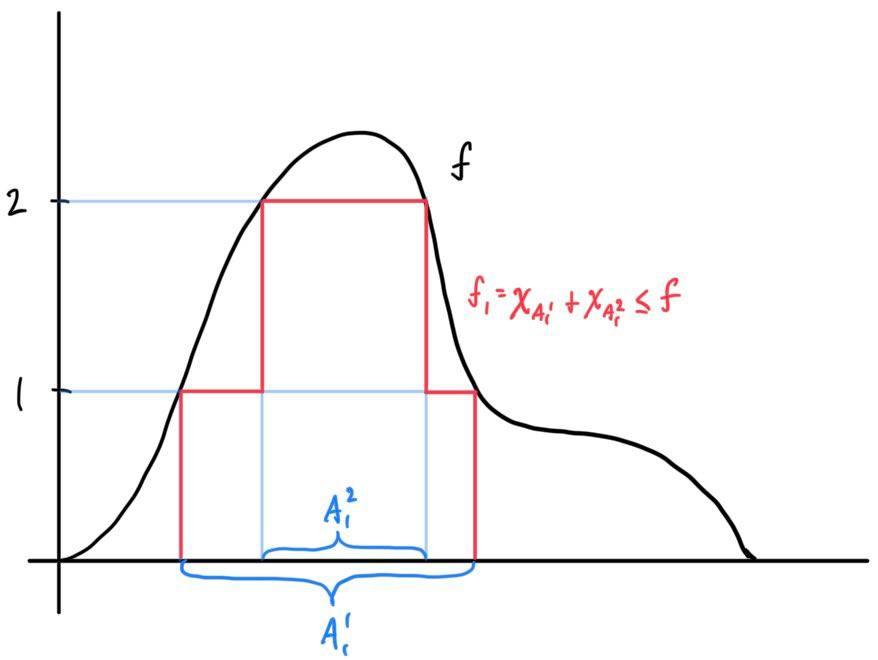
\includegraphics[scale=0.23]{img/Lebesgue_1.jpg}
  \end{center}
  Doing this again with finer subintervals of the codomain gives us, with $f_2 = \chi_{A_2^1} + \chi_{A_2^2} + \chi_{A_2^3} + \chi_{A_2^4} \leq f$. 
  \begin{center}
      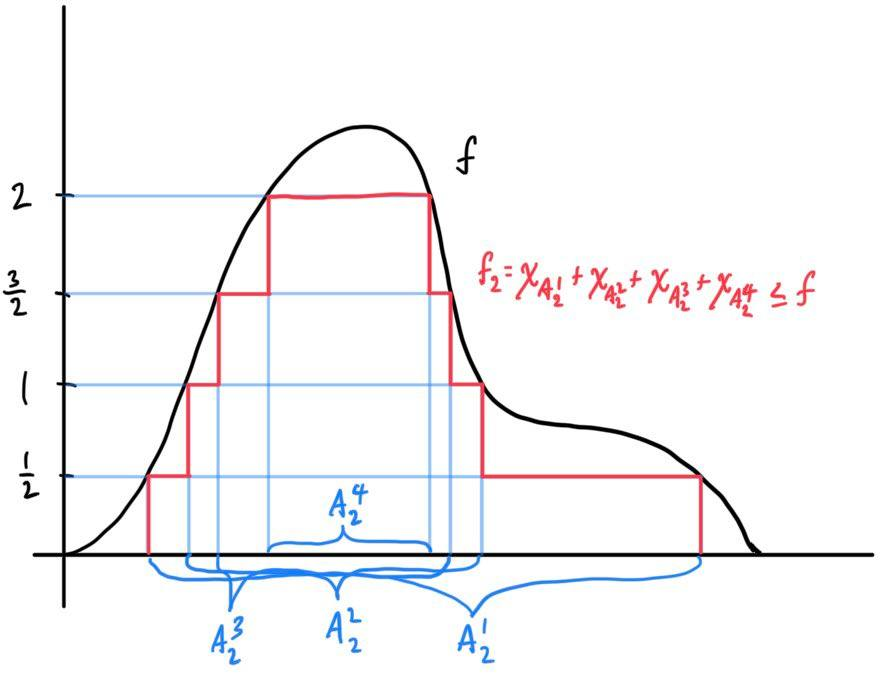
\includegraphics[scale=0.23]{img/Lebesgue_2.jpg}
  \end{center}
  and in general, we have $f_k = \sum_{j=1}^\infty \frac{1}{2^{k-1}} \chi_{A^j_k}$. But we said a simple function is a \textit{finite} sum, and if $\infty$ is in the range of $f$, then this becomes a problem. We can quickly fix this by just truncating the summation at a certain point in the codomain ($f_1$ only considers intervals up to $1$, $f_2$ up to $2$ and so on), ultimately giving us 
  \[f_k = \sum_{j=1}^{k 2^{k-1}} \frac{1}{2^{k-1}} \chi_{A^j_k} \]
\end{proof}

\subsection{Lebesgue Integral}

Finally, we can learn how to integrate. We require the positiveness condition on $f$ below because our previous theorem on approximating arbitrary functions with simple measurable functions $f_k$ requires that it be positive, too. 

\begin{definition}[Lebesgue Integral of Positive Simple Functions]
  If $f = \sum_{k=1}^n c_k \chi_{A_k}$ is a positive simple Lebesgue measurable function on measure space $(X, \mathcal{A}, \mu)$, then the \textbf{Lebesgue integral} of $f$ is 
  \[\int f \, d\mu = \sum_{k=1}^n c_k \mu(A_k)\]
\end{definition}

This Lebesgue integral agrees with the Riemann integral for step functions. Let $c_1, \ldots, c_n \in [0, \infty)$ and $a = x_0 < x_1 < \ldots < x_n = b$ be a partition. Let $f: [a, b] \longrightarrow [0, \infty]$ be a step function taking the value $c_i$ on the interval $(x_{i-1}, x_i)$ for $i = 1, \ldots, n$. Then the Riemann integral of $f$ is simply 
\[\int f(x) \,dx = \sum_{i=1}^n c_k |x_i - x_{i-1}|\]
The Lebesgue integral is 
\begin{align*}
  \int f \, d \mu & = \sum_{i=1}^n c_i \mu((x_{i-1}, x_i)) + \sum_{j=0}^n f(x_j) \mu(\{x_j\}) \\
  & = \sum_{i=1}^n c_k |x_i - x_{i-1}|
\end{align*}
which agrees with the Riemann integral. In the Riemann integral, we write $dx$ to indicate the variable that is being integrated over, but in the Lebesgue integral, we write $d \mu$, the measure which we are integrating over. Therefore, there are many possible values that can come out of a Lebesgue integral of a certain function, while a Riemann integral outputs only one value if exists. 

\begin{example}
  Consider the simple function (consisting of one characteristic function) $\chi_{\mathbb{Q} \cap [0, 1]}$. $\mathbb{Q} \cap [0, 1]$ is a Lebesgue measurable set of $\mathbb{R}$, and we have $\chi_{\mathbb{Q} \cap [0, 1]} \geq 0$, so its Lebesgue integral is given by the above definition: 
  \[\int_{\mathbb{R}} \chi_{\mathbb{Q} \cap [0, 1]} \, d\lambda = 1 \cdot \lambda(\mathbb{Q} \cap [0, 1]) = 0\]
\end{example}

\begin{definition}[Lebesgue Integral on Positive Measurable Functions]
  If $f: (X, \mathcal{A}, \mu) \longrightarrow [0, \infty]$ is measurable, then 
  \[\int_X f \, d\mu = \sup \Big\{ \int g\, d\mu \,\Big|\, g \text{ simple }, g \leq f\Big\}\]
\end{definition}

Unlike Riemann integration, which looks at both the supremum and infimum of integrals of simple functions, Lebesgue integration only looks at the supremum, given that $f$ is nonnegative, so for all these $f$, the Lebesgue integral always exists. Defining Lebesgue integration for all real-valued functions, requires a simple extension. 

\begin{definition}[Lebesgue Integral]
  Given a function $f: (X, \mathcal{A}, \mu) \longrightarrow \mathbb{R}$, we can split $f$ into a positive and negative part: 
  \[f = f^+ - f^-\]
  where $f^+ = \max(f, 0)$ and $f^- = \max(-f, 0)$. Then, the Lebesgue integral of $f$ is 
  \[\int f \, d \mu = \int f^+ \, d\mu - \int f^- \, d\mu\]
  given that at least one of these integrals is finite. If one is infinite and the other is finite, then we can call it infinite. If we have \textit{both} infinite integrals, then the integral doesn't exist. It has the properties: 
  \begin{enumerate}
    \item Monotonicity: 
    \[g \leq f \implies \int g \, d\mu \leq \int f\, d\mu\]
    \item Scalar Multiplication: 
    \[\int c f \, d\mu = c \int f \, d\mu\]
    \item Addition:
    \[\int f + g \, d\mu = \int f \,d\mu + \int g \,d\mu\]
  \end{enumerate}
\end{definition}

Since $|f| = f^+ + f^-$, $f$ is also Lebesgue integrable if 
\[\int |f| \, d\mu < \infty \]
since by triangle inequality, we have 
\[\bigg| \int f \, d\mu \bigg| \leq \int |f| \, d \mu\]

\begin{definition}
  The set of all functions $f: (X, \mathcal{A}, \mu) \longrightarrow \mathbb{R}$ that are Lebesgue integrable is denoted $\mathcal{L}^1(X, \mathcal{A}, \mu; \mathbb{R})$, or for short $\mathcal{L}^1(X, \mathcal{A}, \mu)$. 
\end{definition}

\begin{theorem}
  Suppose $f: (\mathbb{R}, \mathcal{A}, \mu) \longrightarrow \mathbb{R}$ is $0$ almost everywhere. Then $f$ is Lebesgue integrable with 
  \[\int_\mathbb{R} f \, d\mu = 0 \]
  If $g: \mathbb{R} \longrightarrow \mathbb{R}$ is such that $f = g$ $\mu$-almost everywhere, then
  \[\int_\mathbb{R} f\, d\mu = \int_\mathbb{R} g \, d\mu\]
\end{theorem}

\subsection{Monotone Convergence Theory}

From now on, we will assume that all spaces $X$ are measure spaces $(X, \mathcal{A}, \mu)$ and all functions $f$ are measurable functions. The huge problem with Riemann integrals is that this theorem doesn't hold, but it is the case for Lebesgue integration. 

\begin{theorem}[Monotone Convergene Theorem (MCT)]
  Given a nondecreasing sequence of measurable functions $f_1 \leq f_2 \leq f_3 \leq \ldots : X \longrightarrow [0, \infty]$, its limit $\lim_{k \rightarrow \infty} f_k$ always exists (since $f_k$ is nondecreasing), is measurable, and 
  \[\int \lim_{k \rightarrow \infty} f_k \, d\mu = \lim_{k \rightarrow \infty} \int f_k \, d\mu\]
  This allows us to integrate the limit of nice functions $f_k$ by integrating these $f_k$ first and then finding what the values converge to. 
\end{theorem}

\subsection{Riemann vs Lebesgue Integral}

\begin{theorem}
  $f: \mathbb{R} \longrightarrow \mathbb{R}$ is Riemann integrable iff it is continuous $\lambda$ almost everywhere. If so, then $f$ is Lebesgue measurable and 
  \[\int_{[a, b]} f \,d\lambda = \int_a^b f \, dx\]
  for all $a < b \in \mathbb{R}$. 
\end{theorem}

\end{document}

